\section{Произволный домен}

В качестве произвольного домена для анализа был выбран ru.sharelatex.com. 

\begin{figure}[H]
    \centering
    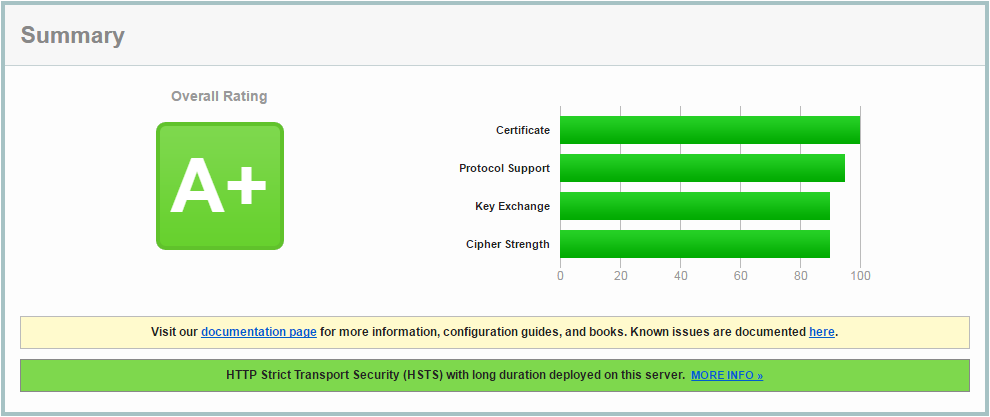
\includegraphics[width=\textwidth]{resources/03_summary.png}
    \caption{Сводка по домену ru.sharelatex.com}
    \label{fig:03-summary}
\end{figure}

Оценка домена была улучшена до \code{A+} поскольку включена поддержка HSTS с достаточно длинным периодом времени.

Ниже приведена таблица рассшифровок шифров, доступных для использования на рассматриваемом домене. Колонки таблицы зашифрованы 
согласно нотации, представленной в разделе \ref{ssct:best-practices.configuration}.

\begin{table}[H]
    \centering
    \begin{tabular}{c|c|c|c|c|c}
        \textbf{P} & \textbf{KEA} & \textbf{AA} & \textbf{MEA} & \textbf{Мощность} & \textbf{HA} \\ 
        \hline
        TLS & ECDHE & RSA & AES\_128\_GCM & $128$ & SHA256 \\
        TLS & ECDHE & RSA & AES\_128\_CBC & $128$ & SHA256 \\
        TLS & ECDHE & RSA & AES\_128\_CBC & $128$ & SHA \\
        TLS & RSA & RSA & AES\_128\_GCM & $128$ & SHA256 \\
        TLS & RSA & RSA & AES\_128\_CBC & $128$ & SHA256 \\
        TLS & RSA & RSA & AES\_128\_CBC & $128$ & SHA \\
        TLS & ECDHE & RSA & AES\_256\_GCM & $256$ & SHA384 \\
        TLS & ECDHE & RSA & AES\_256\_CBC & $256$ & SHA384 \\
        TLS & ECDHE & RSA & AES\_256\_CBC & $256$ & SHA \\
        TLS & RSA & RSA & AES\_256\_GCM & $256$ & SHA384 \\
        TLS & RSA & RSA & AES\_256\_CBC & $256$ & SHA256 \\
        TLS & RSA & RSA & AES\_256\_CBC & $256$ & SHA \\
        TLS & ECDHE & RSA & 3DES\_EDE\_CBC & $112$ & SHA \\
        TLS & RSA & RSA & 3DES\_EDE\_CBC & $112$ & SHA \\
    \end{tabular}
    \caption{Шифры, доступные на ru.sharelatex.com}
    \label{tbl:03-cipher-suits}
\end{table}

Приведем теперь разбор некоторых деталий реализации протокола на рассматриваемом домене по категориям, рассмотренным в секции 
\ref{ssct:best-practices.protocol-details}

\begin{table}[H]
    \centering
    \begin{tabular}{c|c}
        \hline
        \multicolumn{2}{c}{\textbf{Уязвимости}} \\ \hline
        \textbf{Уязвимость} & \textbf{Уязвим} \\ \hline
        \textbf{DROWN} & Нет \\
        \textbf{BEAST} & Да, со стороны сервера \\
        \textbf{POODLE} & Нет \\
        \textbf{Атака на понижение версии} & Нет \\
        \textbf{Heartbleed} & Нет \\
        \textbf{OpenSSL CCS} & Нет \\
        \textbf{OpenSSL Padding Oracle} & Нет \\ \hline
        \multicolumn{2}{c}{\textbf{Опции}} \\ \hline
        \textbf{Опция} & \textbf{Включена} \\ \hline 
        \textbf{Безопасное переподключение} & Да \\ 
        \textbf{Сжатие данных} & Нет \\ 
        \textbf{Пульс} & Да \\ 
        \textbf{Продожительная защищенность} & Да \\ 
        \textbf{ALPN} & Нет \\ 
        \textbf{NPN} & Да (HTTP/1.1) \\ 
        \textbf{Возобновление сессии (кэширование)} & Нет \\
        \textbf{Возобновление сессии (билеты)} & Да  \\
        \textbf{OCSP сшивание} & Нет  \\
        \textbf{HSTS} & Да \\ 
        \textbf{HPKP} & Нет \\ 
        \textbf{Отказ в длинном рукопожатии} & Нет \\ 
        \textbf{Отказ от версии} & Нет \\ 
    \end{tabular}
    \caption{Детали реализации протокола на ru.sharelatex.com}
    \label{03-protocol-details}
\end{table}

Настройки данного домена достаточно аналогичны настройкам домена из раздела <<Лучший за последнее время>>, рассматриваемый в данной
работе ранее. Отличие заключается в том, что ru.sharelatex.com более полно поддерживает продолжительную защищенность и принудительную
защищенность транспортного уровня.